\documentclass[UTF8,12pt]{article}

\usepackage[utf8]{inputenc}
\usepackage{ctex}
\usepackage{amsmath,amsfonts,amssymb}
\usepackage{graphicx,epsfig,subfig}
\usepackage{makeidx,hyperref}
\usepackage{geometry}
\usepackage{listings}
\usepackage[linesnumbered,boxed]{algorithm2e}
\usepackage{xcolor}

\geometry{scale=0.8}

%\setlength{\lineskip}{\baselineskip}
\setlength{\parskip}{0.5\baselineskip}

\title{Anderson局部化实验报告2}
\author{flag}
\date{\today}

\begin{document}
    
\maketitle

\section{探究参数何时最优}

\subsection{$\alpha$的选取}

我们先从一维的简单情况开始。一维区间分成20段,K=1000,V是均匀分布的随机数,Neumann边界条件。选取$x_0$为0.5 对不同的$\alpha$模拟。如图\ref{fig1}

\begin{figure}[htbp]
    \centering
    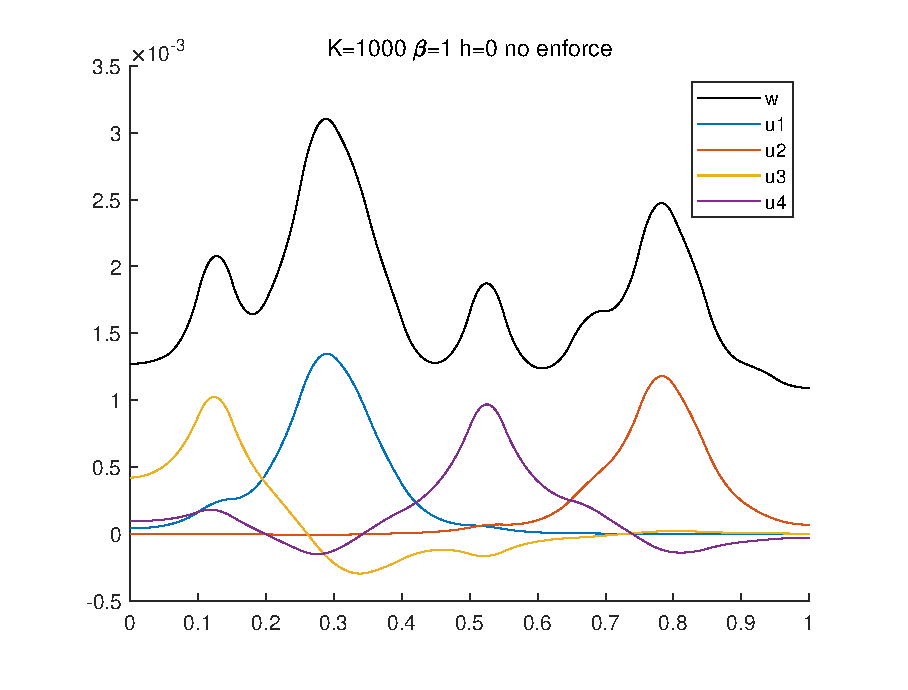
\includegraphics[width=0.3\linewidth]{pic/ua0}
    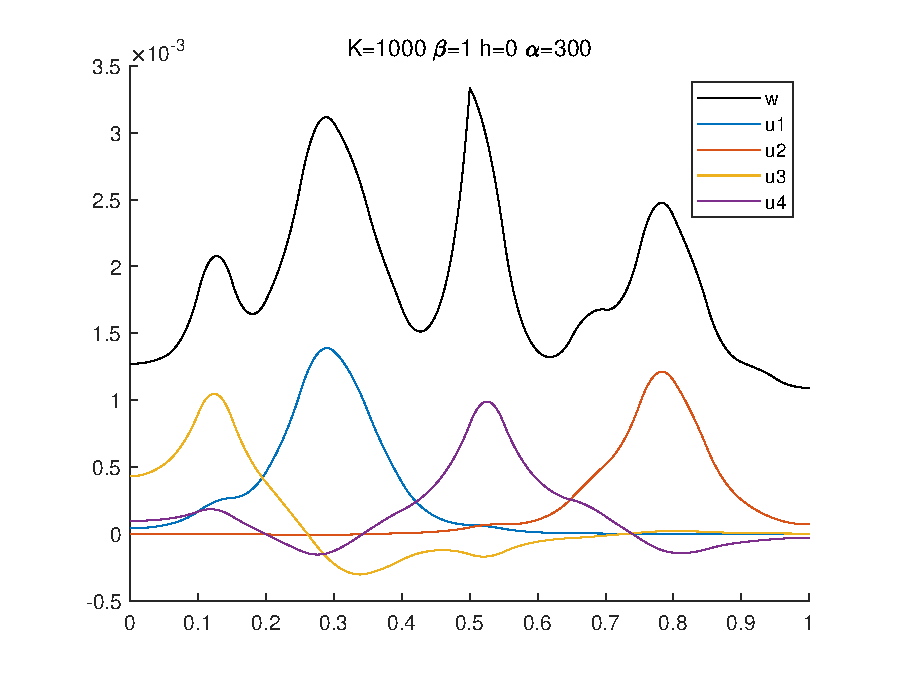
\includegraphics[width=0.3\linewidth]{pic/ua300} \\
    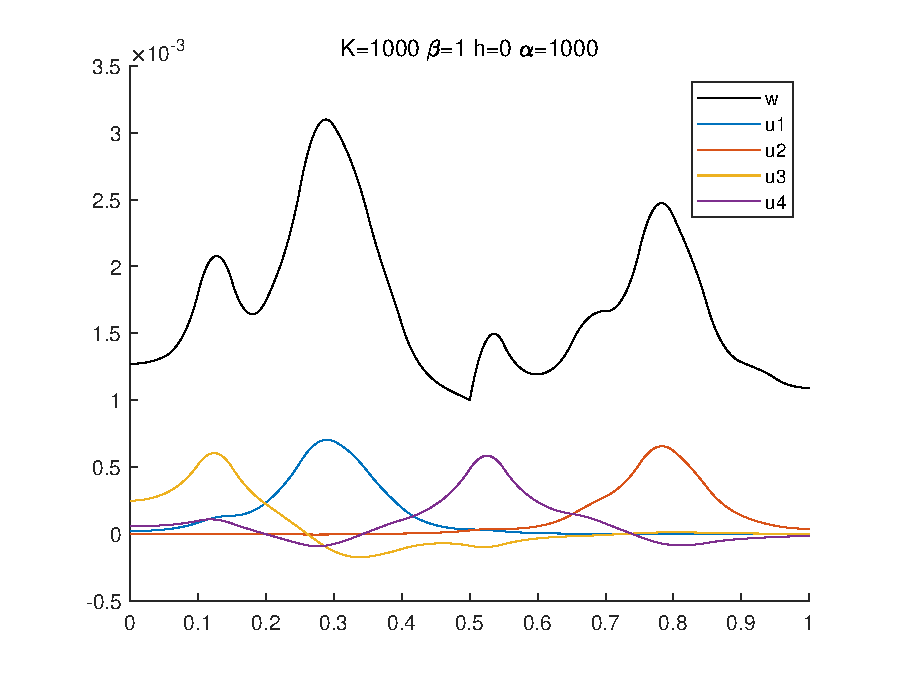
\includegraphics[width=0.3\linewidth]{pic/ua1000}
    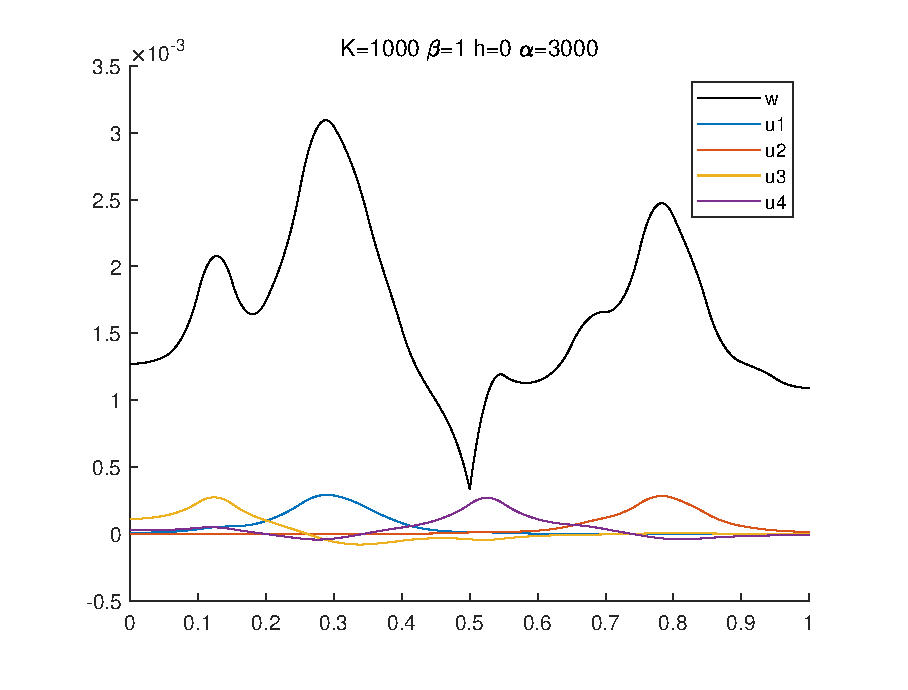
\includegraphics[width=0.3\linewidth]{pic/ua3000}
    \label{fig1}
\caption{一维,不同alpha下的表现}
\end{figure}

可以看到,在$x_0$附近landscape会间断。我们希望的情况是下面彩色的线和上面黑色的线比较靠近。可以看出,没有enforce的landscape是四幅图里最优的。

把四条landscape画在一起,发现强制的边界仅仅改变了$x_0$附近的函数值,对更远的地方就没有效果了。在二维情况,这种现象特别特别明显。如图\ref{fig2}。图中二维分割成$20 \times 20$的小块,$\alpha = 200$其他参数同上。

\begin{figure}[htbp]
    \centering
    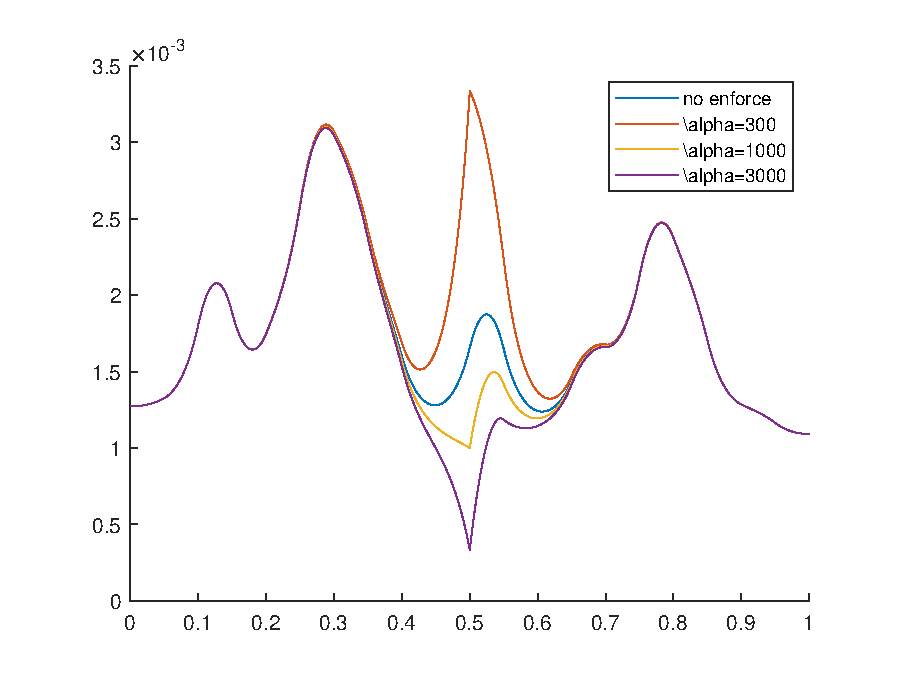
\includegraphics[width=0.3\linewidth]{pic/nouse1d}
    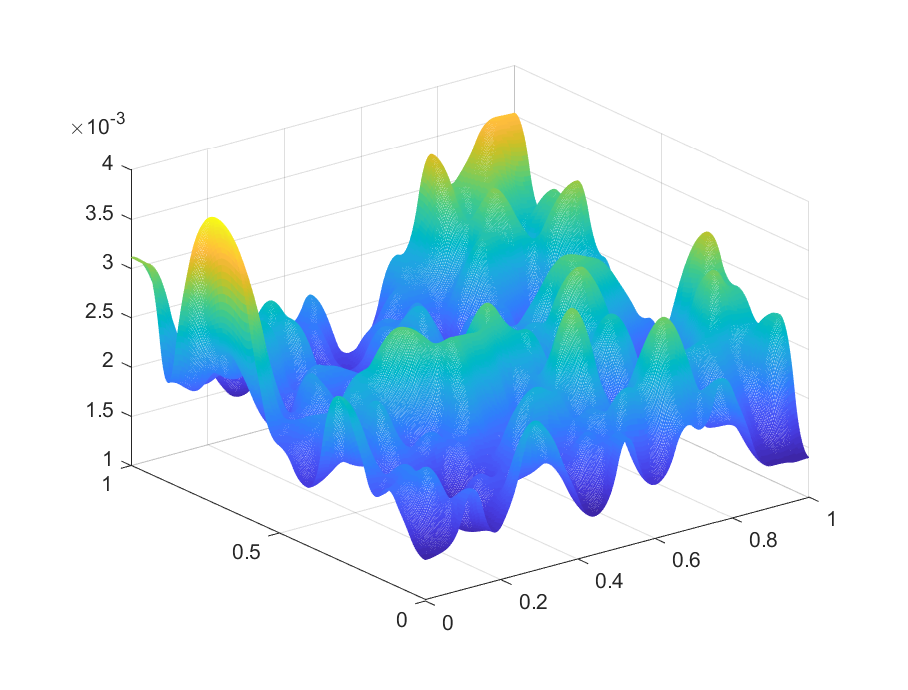
\includegraphics[width=0.3\linewidth]{pic/nouse2d1}
    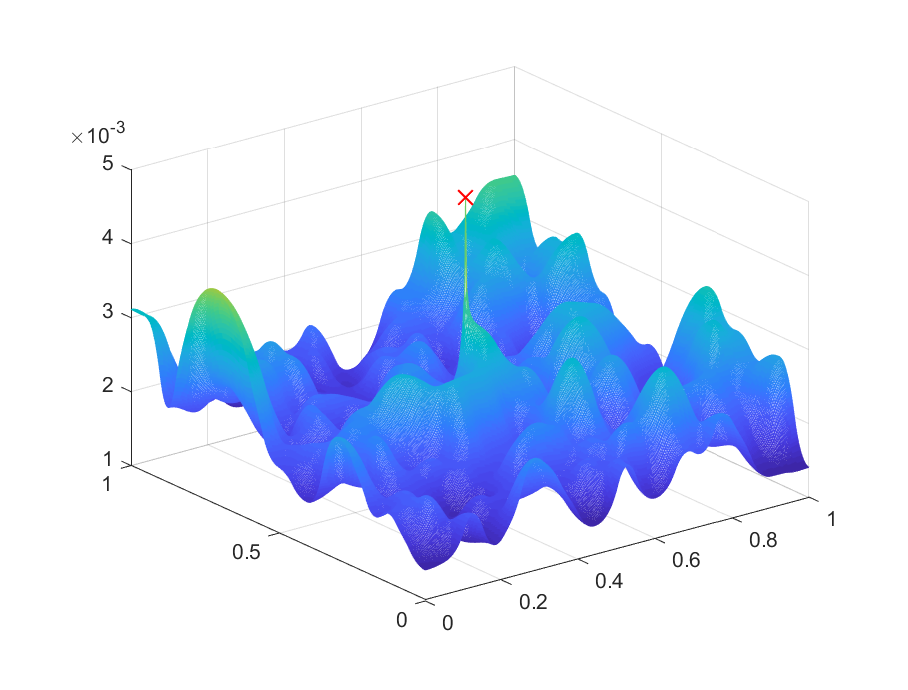
\includegraphics[width=0.3\linewidth]{pic/nouse2d2}
    \label{fig2}
\caption{左图是一维的情况,中间是no enforce的二维曲面,右边是把(0.5, 0.5)处强行设成1/200的曲面。红叉下面那个特别细的就是enforce对它的影响。}
\end{figure}

综合以上现象,我觉得$\alpha$直接选成landscape最大值的倒数就好。

\subsection{$\beta$的选取}

首先在一维情况下实验,Robin边界条件,取h=1,其他参数同上。结果如图\ref{fig3}
\begin{figure}[htbp]
    \centering
    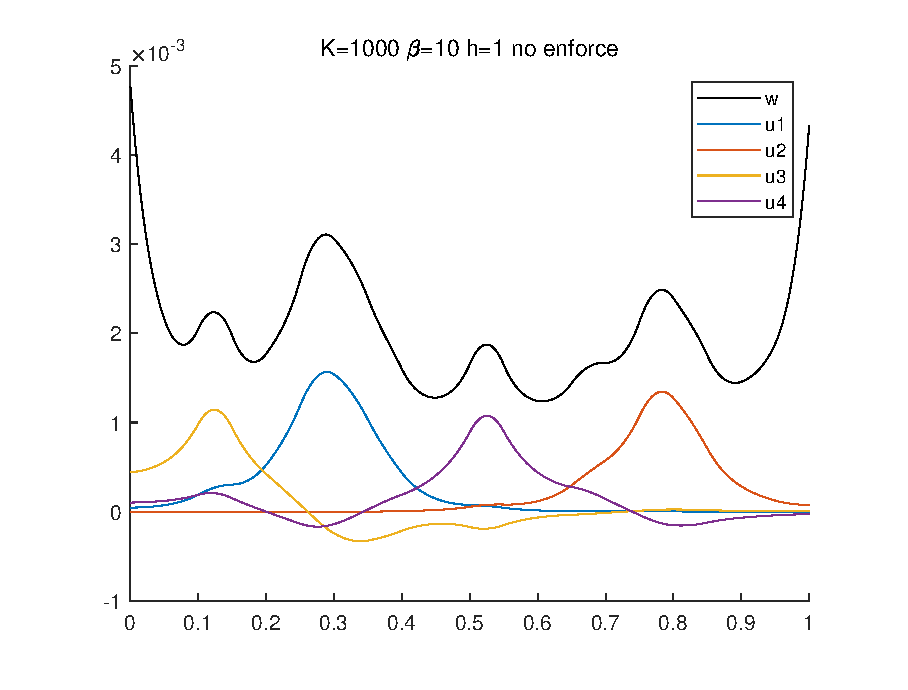
\includegraphics[width=0.3\linewidth]{pic/h1b10}
    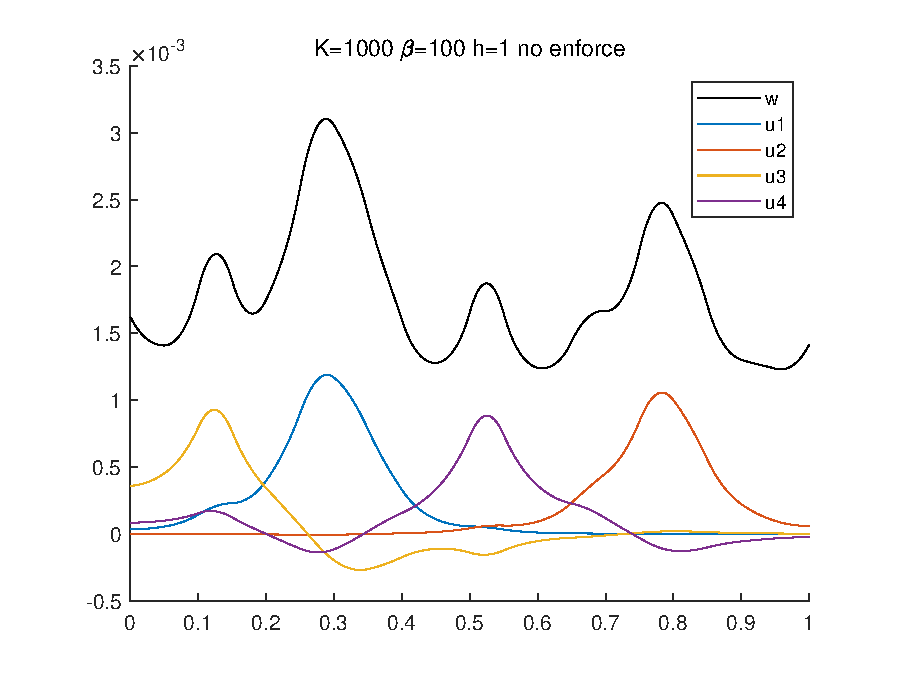
\includegraphics[width=0.3\linewidth]{pic/h1b100}
    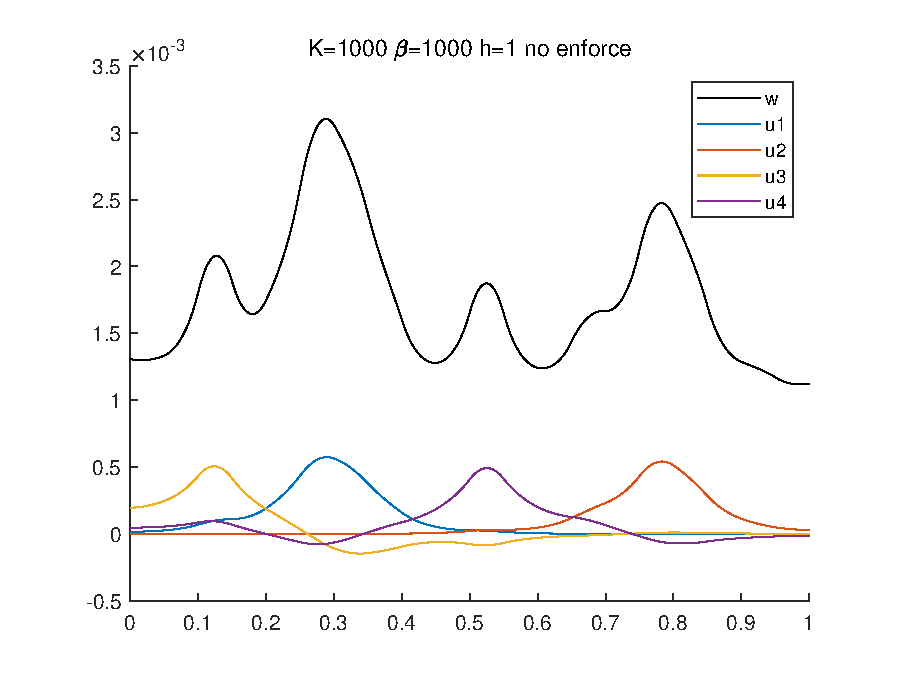
\includegraphics[width=0.3\linewidth]{pic/h1b1000}
    \label{fig3}
\caption{beta对结果的影响}
\end{figure}

从图中可以看出,$\beta$不能太小,否则边界会翘起来,也不能太大,否则不等式就不精确了。之前猜测$\beta$应该大概取成$Kh$,现在看起来并不是这样。

同样,$\beta$的选取仅仅影响landscape在边界附近的性质,对内部影响比较小。如图\ref{fig4}

\begin{figure}[htbp]
    \centering
    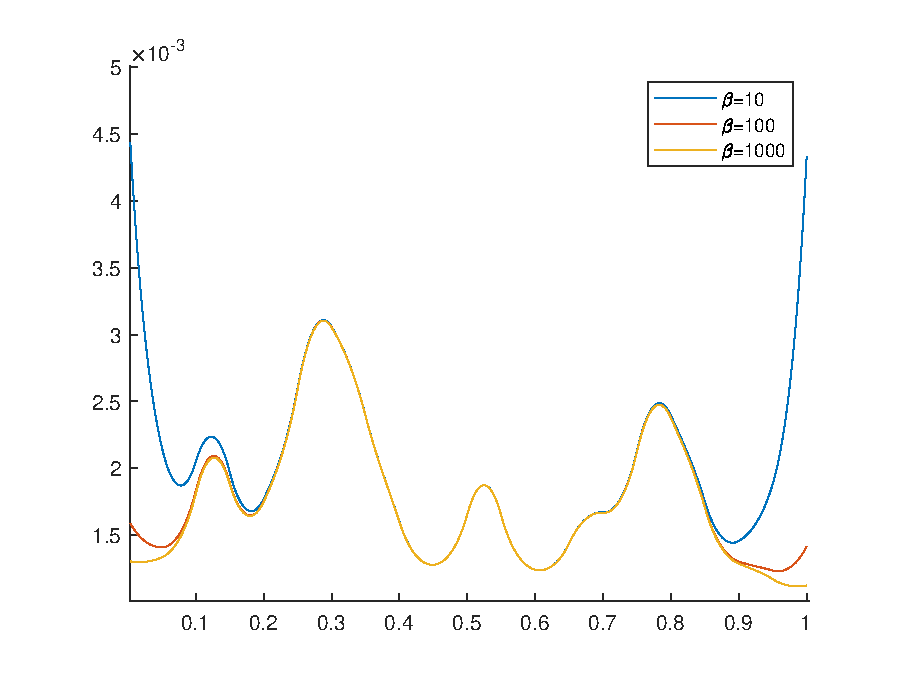
\includegraphics[width=0.4\linewidth]{pic/nouseb1d}
    \label{fig4}
\caption{beta对结果的影响}
\end{figure}

对于什么样的参数是“最优”,并没有一个确切的有指标刻画的标准。对于$\beta$具体取什么样的值比较好,现在只能说可以在边界不会翘起来的情况下,可以尽量取得小一点。

\section{画出valley line}

目前得valley line画出来是这样。
\begin{figure}[htbp]
    \centering
    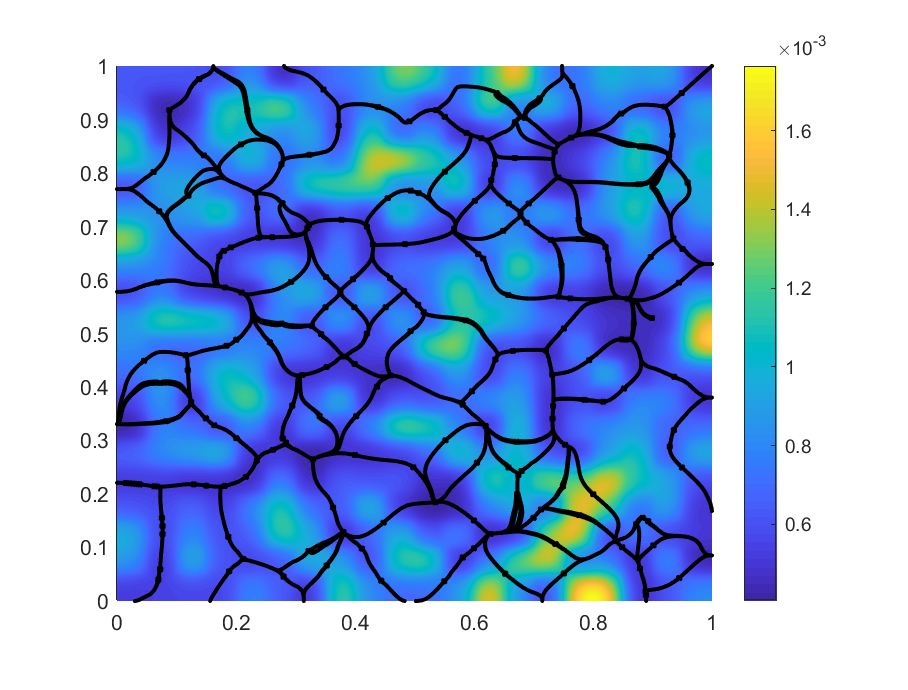
\includegraphics[width=0.4\linewidth]{pic/vline2}
    \label{figv1}
\caption{K=3000,均匀分布}
\end{figure}

画出其中大于$1/(2\lambda_1)$的valleyline是这样。
\begin{figure}[htbp]
    \centering
    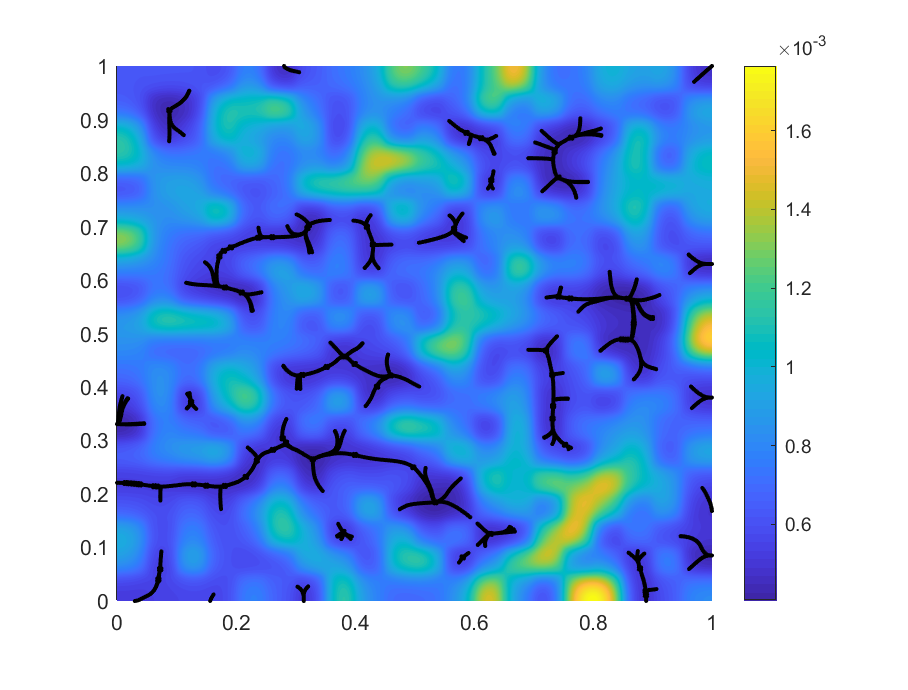
\includegraphics[width=0.4\linewidth]{pic/vline3}
    \label{figv2}
\caption{K=3000,均匀分布}
\end{figure}

\section{不同边界条件下的比较}

在实验中我们发现,边界条件是Dirichlet还是导数型的,主要影响landscape的边界,对landscape的内部影响较小。对eigenmode的影响就比较大,因为原来不会聚集到边界的峰有可能聚集到边界了。

还是先看一维的情况,在一个特定的V下模拟,这里的V故意在边界选取得比较小,能够突出局部化到边界的效果。如图\ref{fig6}
\begin{figure}[htbp]
    \centering
    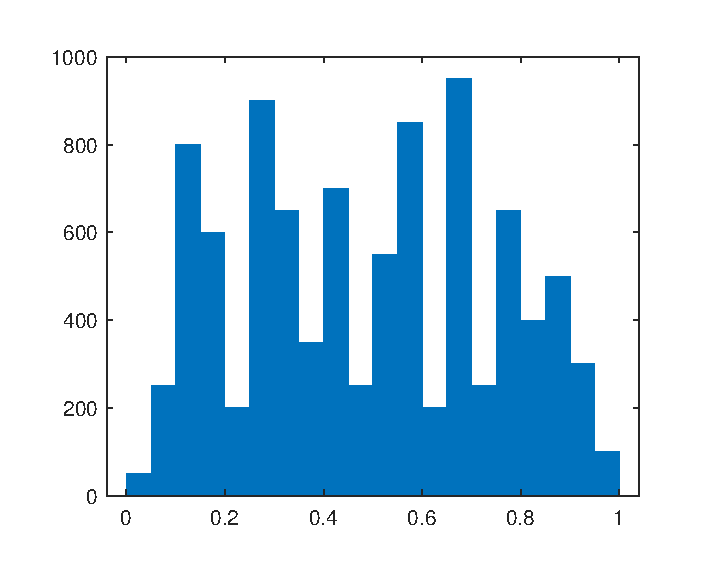
\includegraphics[width=0.4\linewidth]{pic/bdnu1}
    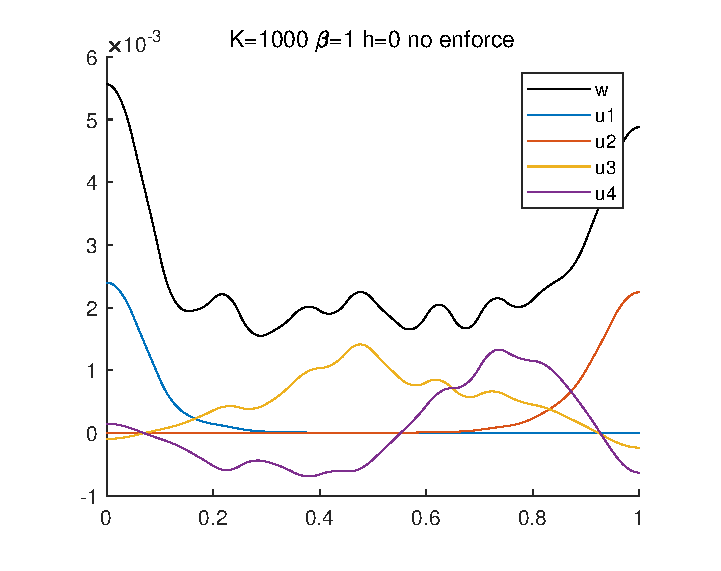
\includegraphics[width=0.4\linewidth]{pic/bdnu2} \\
    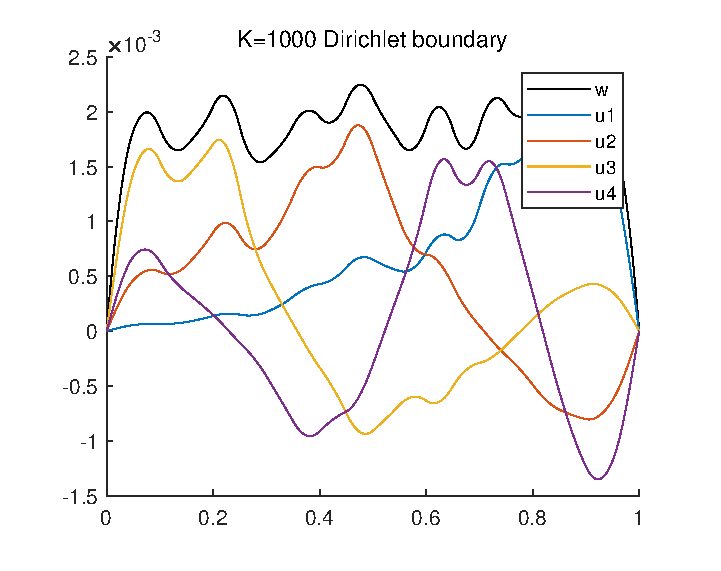
\includegraphics[width=0.4\linewidth]{pic/bdnu3}
    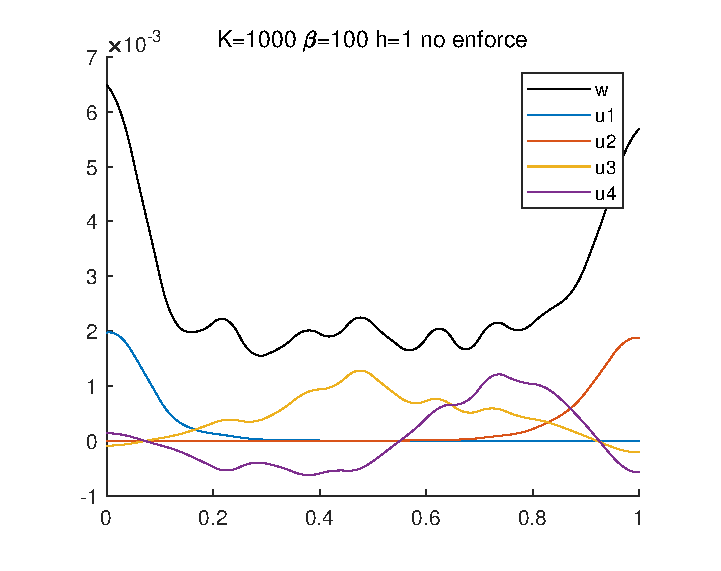
\includegraphics[width=0.4\linewidth]{pic/bdnu4}
    \label{fig6}
\caption{左上为V,剩下三个是不同边界条件下的模拟结果}
\end{figure}

这三个eigenmode很不一样,尤其是Dirichelt和Neumann边界的,相差很多。但是把它们的landscape画在一起,就会发现在内部很相似。图\ref{fig7}中比较了不同边界条件下的landscape。
\begin{figure}[htbp]
    \centering
    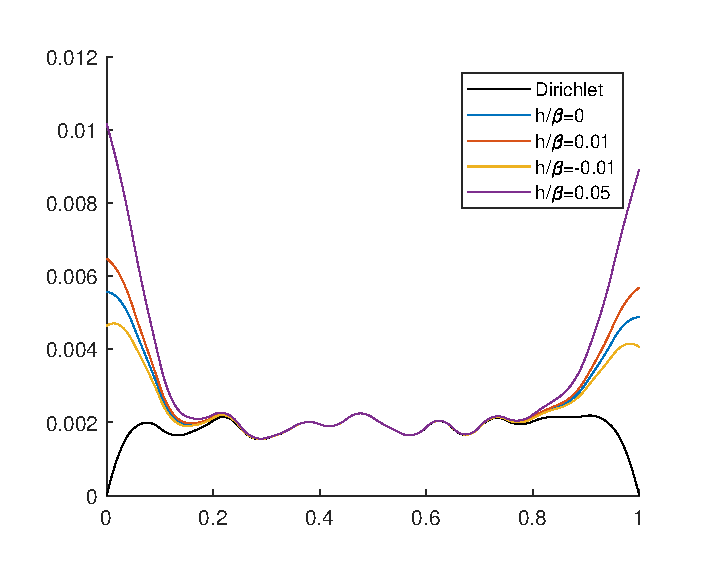
\includegraphics[width=0.4\linewidth]{pic/bdnu5}
    \label{fig7}
\caption{不同边界条件下的landscape}
\end{figure}

二维的也一样。二维的曲面画在一起就乱了,我们只能画切面图。如图\ref{fig8}。landscape在内部差不多。在y=0和y=1的时候就不一样了。
\begin{figure}[htbp]
    \centering
    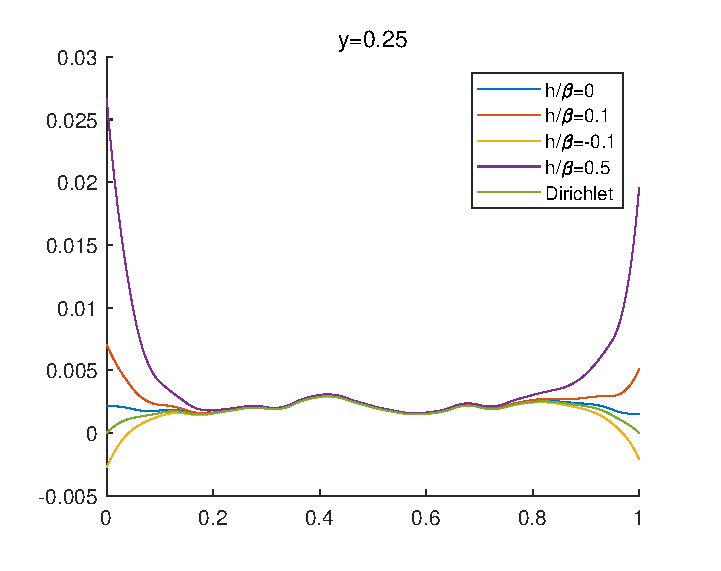
\includegraphics[width=0.3\linewidth]{pic/bdny25}
    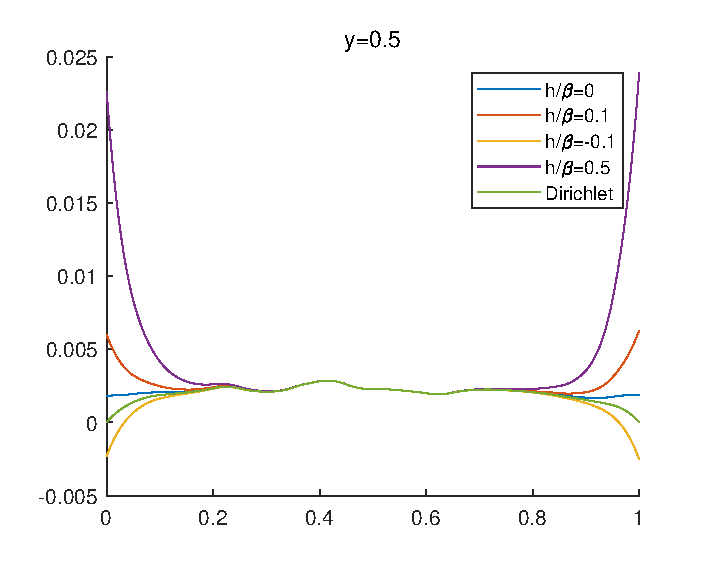
\includegraphics[width=0.3\linewidth]{pic/bdny5}
    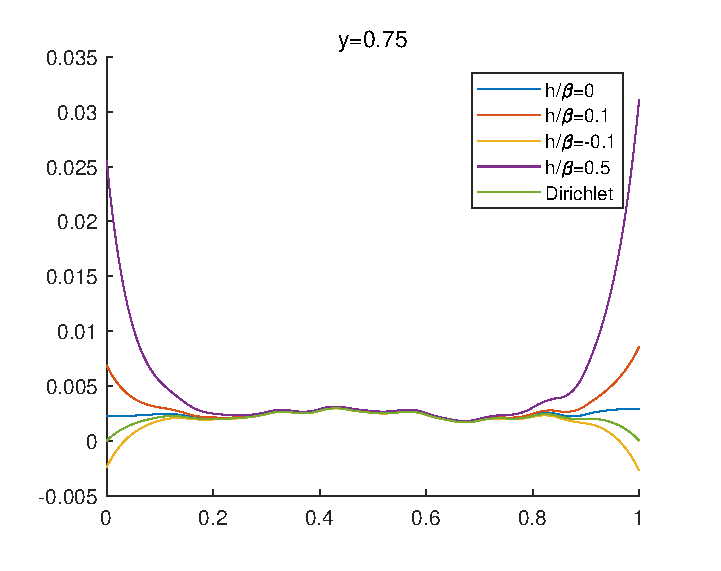
\includegraphics[width=0.3\linewidth]{pic/bdny75}
    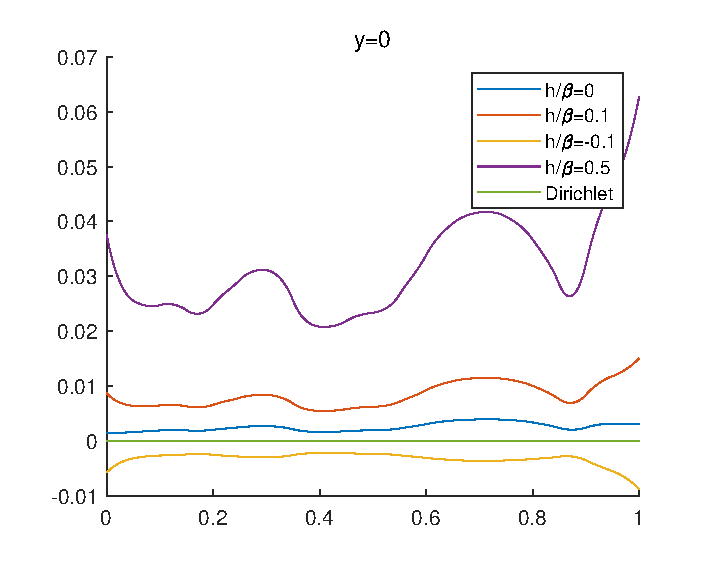
\includegraphics[width=0.3\linewidth]{pic/bdny0}
    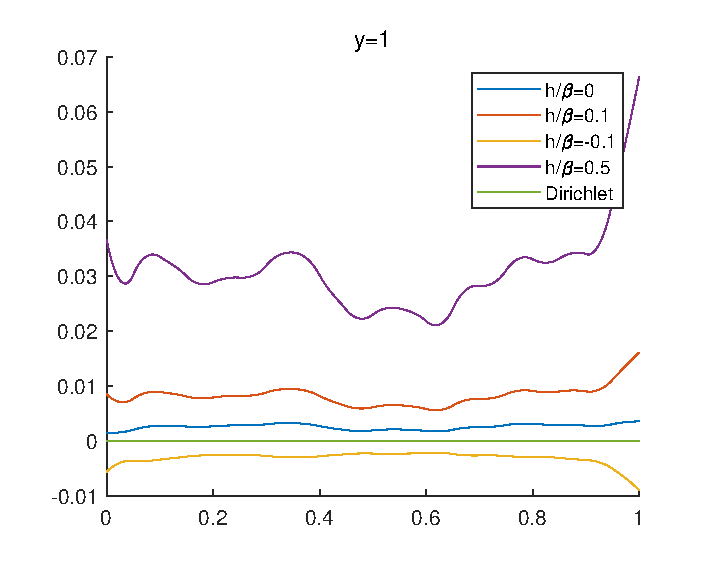
\includegraphics[width=0.3\linewidth]{pic/bdny1}
    \label{fig8}
\caption{二维不同边界条件下的landscape}
\end{figure}


之前有一个问题是当localize的位置在边界时,要如何选取$\beta$的值,这时的结果会不会有变化。我们用同样的势函数,换不同的$\beta$模拟。结果如图\ref{fig9}。得到的结果和原来差不多。由于在最终的不等式里出现的是$\beta$和特征值相加,所以$\beta$选取和特征值在同一数量级的数就差不多。
\begin{figure}[htbp]
    \centering
    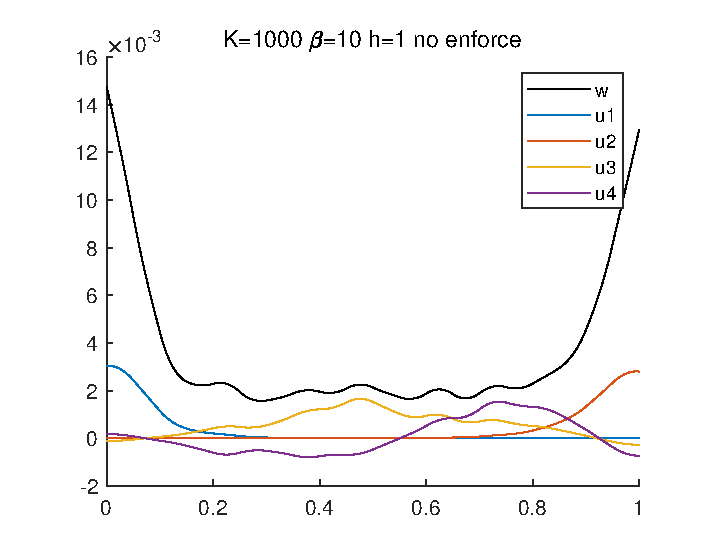
\includegraphics[width=0.3\linewidth]{pic/bdb2}
    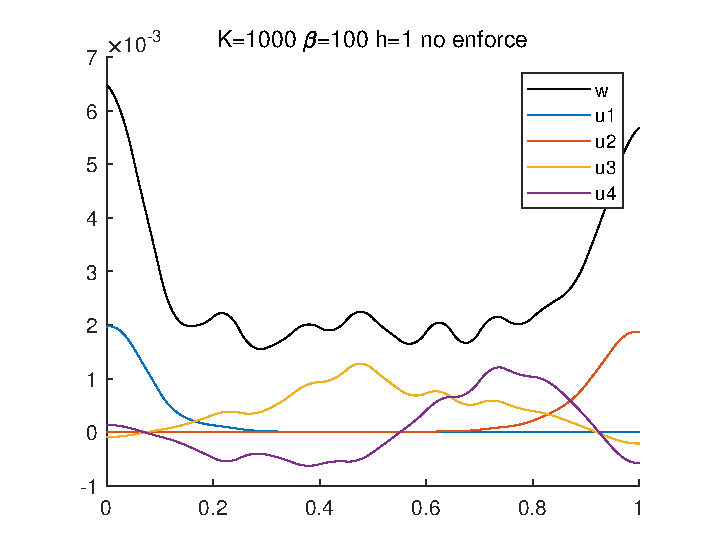
\includegraphics[width=0.3\linewidth]{pic/bdb3}
    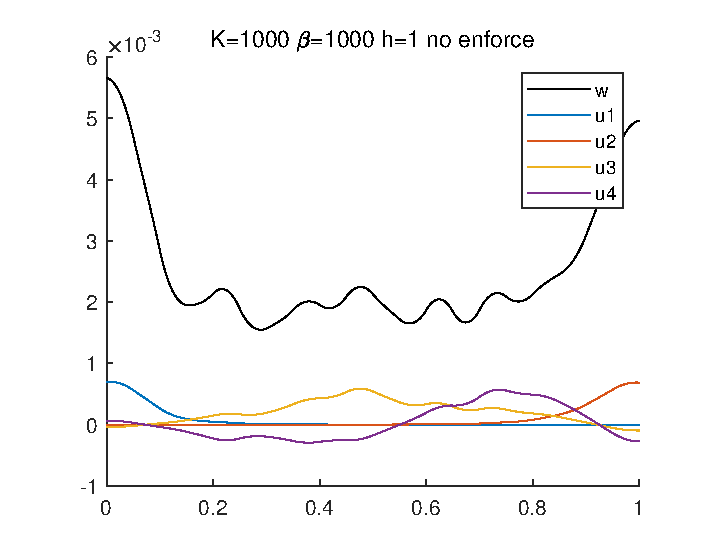
\includegraphics[width=0.3\linewidth]{pic/bdb4}
    \label{fig9}
\caption{localize到边界的landscape}
\end{figure}



\end{document}